


\tikzset{every picture/.style={line width=0.75pt}} %set default line width to 0.75pt        

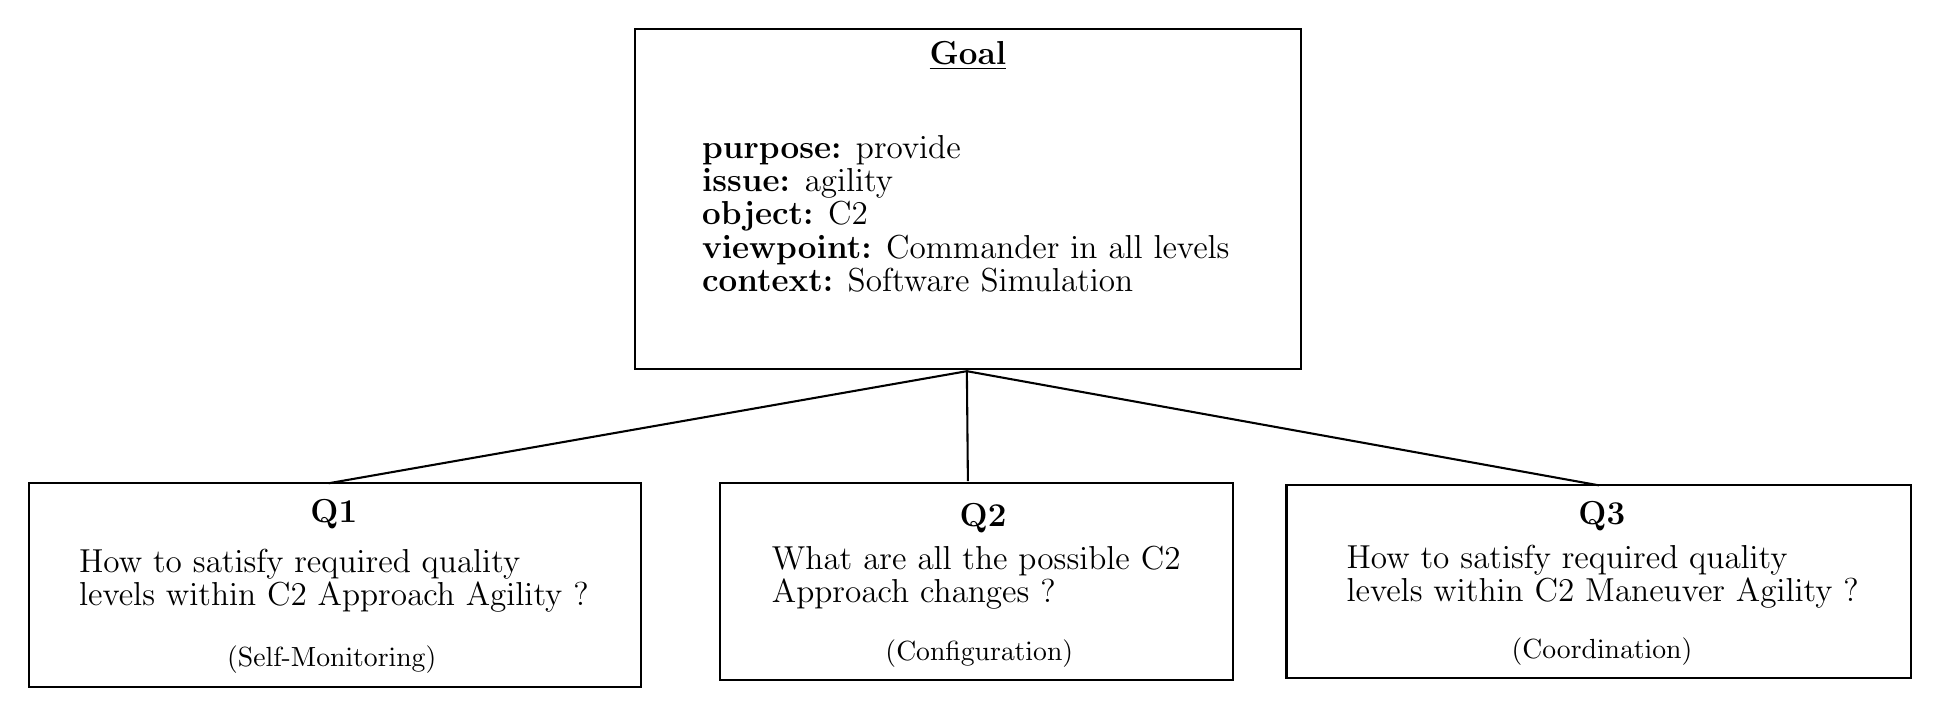
\begin{tikzpicture}[x=0.75pt,y=0.75pt,yscale=-1,xscale=1]
%uncomment if require: \path (0,334); %set diagram left start at 0, and has height of 334

%Flowchart: Process [id:dp9228173025001839] 
\draw   (295,2) -- (616,2) -- (616,166) -- (295,166) -- cycle ;
%Shape: Rectangle [id:dp9468174970136011] 
\draw   (609,222) -- (910,222) -- (910,315) -- (609,315) -- cycle ;
%Shape: Rectangle [id:dp09665993774558346] 
\draw   (3,221) -- (298,221) -- (298,319) -- (3,319) -- cycle ;
%Shape: Rectangle [id:dp4625317111731858] 
\draw   (336,220.67) -- (583,220.67) -- (583,316) -- (336,316) -- cycle ;
%Straight Lines [id:da1961523796551078] 
\draw    (455,167) -- (147.5,221) ;


%Straight Lines [id:da6120336423295578] 
\draw    (455,167) -- (759.5,222) ;


%Straight Lines [id:da223601999954537] 
\draw    (455,167) -- (455.5,220) ;



% Text Node
\draw (455.5,15) node  [font=\normalsize] [align=left] {\textbf{\underline{{\large Goal}}}};
% Text Node
\draw (150,236) node   [align=left] {\textbf{{\large Q1}}};
% Text Node
\draw (150,268) node   [align=left] {{\large How to satisfy required quality }\\{\large levels within C2 Approach Agility ?}};
% Text Node
\draw (459.5,266.67) node   [align=left] {{\large What are all the possible C2}\\{\large Approach changes ?}};
% Text Node
\draw (761.33,266) node   [align=left] {{\large How to satisfy required quality }\\{\large levels within C2 Maneuver Agility ?}};
% Text Node
\draw (760.92,237) node   [align=left] {\textbf{{\large Q3}}};
% Text Node
\draw (462.83,237.67) node   [align=left] {\textbf{{\large Q2}}};
% Text Node
\draw (454.5,91) node   [align=left] {{\large \textbf{purpose:} provide}\\{\large \textbf{issue:} agility}\\{\large \textbf{object:} C2}\\{\large \textbf{viewpoint:} Commander in all levels}\\{\large \textbf{context:} Software Simulation}};
% Text Node
\draw (461,303) node   [align=left] {(Configuration)};
% Text Node
\draw (149,306) node   [align=left] {(Self-Monitoring)};
% Text Node
\draw (761,302) node   [align=left] {(Coordination)};


\end{tikzpicture}